\documentclass[10pt]{beamer}

\usepackage{pgfplots}
\usepackage{pgfplotstable}
\usepackage{tikz}

\usetikzlibrary{calc}
\usetikzlibrary{shadings}

\usetheme{PSY9511}

\title{Artificial Intelligence in Healthcare}
\subtitle{Identifying neuroimaging endophenotypes with AI}
\author{Esten H. Leonardsen}
\date{07.02.25}

\pgfplotsset{
    discard if not/.style 2 args={
        x filter/.code={
            \edef\tempa{\thisrow{#1}}
            \edef\tempb{#2}
            \ifx\tempa\tempb
            \else
                \def\pgfmathresult{inf}
            \fi
        }
    }
}

\begin{document}
	\begin{frame}
	 	\maketitle
	\end{frame}

    \begin{frame}{Outline}
        \textbf{Plan for the day}
        \begin{enumerate}
            \item Why do we need new imaging phenotypes?
            \item How can we find new phenotypes with AI?
            \item Use case: Explainable AI for dementia
            \item Use case: Pretraining with multitask learning
            \item Use case: Explainable brain age predictions
        \end{enumerate}
    \end{frame}

    \newcommand{\largefeaturespace}[1]{
    \begin{tikzpicture}
        \ifnum#1>4
            \def\xAxisFlip{, x dir=reverse}%
        \else
            \def\xAxisFlip{}%
        \fi

        \ifnum#1=6
            \def\axisTextColor{, x label style={red}}%
        \else
            \def\axisTextColor{}%
        \fi

        \ifnum#1=4
            \def\axisText{, xlabel=Cortical atrophy}%
        \else
            \def\axisText{, xlabel=Feature 1}%
        \fi

        \begin{axis}[
            height=5cm,
            width=5cm,
            xmajorticks=false,
            ymajorticks=false,
            xlabel=Feature 1,
            ylabel=Feature 2,
            ymin=-1.99,
            ymax=3.99,
            xmin=-3,
            xmax=3,
            clip=false,
            \xAxisFlip
            \axisTextColor
            \axisText
        ]
        \addplot[
            only marks,
            mark=*,
            mark options={
                draw=black,
                fill=white,
                scale=1.25
            },
            opacity=0.5,
            discard if not={label}{0}
        ] table [
            col sep=comma,
            x=x,
            y=y
        ] {data/third_feature_space.csv};
        \addplot[
            only marks,
            mark=*,
            mark options={
                draw=black,
                fill=red,
                scale=1.25
            },
            opacity=0.5,
            discard if not={label}{1}
        ] table [
            col sep=comma,
            x=x,
            y=y
        ] {data/third_feature_space.csv};

        \ifnum#1=1
            \node[circle, draw=black, fill=cyan!80, inner sep=2pt,label=below:\textcolor{cyan!80}{\footnotesize{Synthetic}}] at (rel axis cs: 1, 0) {};
        \fi
        \ifnum#1=2
            \node[draw=cyan!80, circle, label=below:\textcolor{cyan}{\footnotesize{?}}] at (axis cs: 2.5890747321766776,1.356842527297071) {};
        \fi
        \end{axis}
    \end{tikzpicture}
}

\newsavebox{\largefeaturespacenone}
\savebox{\largefeaturespacenone}{
    \largefeaturespace{0}
}
\newsavebox{\largefeaturespaceactivation}
\savebox{\largefeaturespaceactivation}{
    \largefeaturespace{1}
}
\newsavebox{\largefeaturespacesaliency}
\savebox{\largefeaturespacesaliency}{
    \largefeaturespace{2}
}
\newsavebox{\largefeaturespaceconcept}
\savebox{\largefeaturespaceconcept}{
    \largefeaturespace{3}
}
\newsavebox{\largefeaturespacelabel}
\savebox{\largefeaturespacelabel}{
    \largefeaturespace{4}
}
\newsavebox{\largefeaturespacetext}
\savebox{\largefeaturespacetext}{
    \largefeaturespace{5}
}
\newsavebox{\largefeaturespacetextred}
\savebox{\largefeaturespacetextred}{
    \largefeaturespace{6}
}

\begin{frame}{How can we understand these learned features?}
    \begin{tikzpicture}
        \node[draw=black] at (-5.25, -3.5) {};
        \node[draw=black] at (5.25, 3.5) {};

        \visible<2>{
            \node[font=\Large\bfseries] at (0, 0) {
                Explainable AI!
            };
        }

        \visible<3>{
            \node[] at (-3, 1) {
                \usebox{\largefeaturespacenone}
            };
        }
        \visible<4-5>{
            \node[] at (-3, 1) {
                \usebox{\largefeaturespaceactivation}
            };
        }

        \visible<5>{
            \node[anchor=north, font=\bfseries, text depth=0] at (2.5, 3.55) {
                Activation maximization
            };
            \node[inner sep=0pt, draw=black] at (2.5, 1) {
                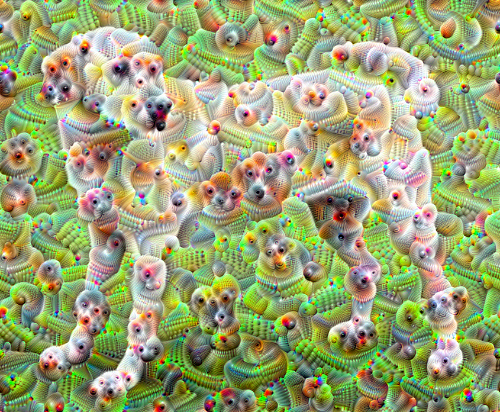
\includegraphics[width=5cm]{data/dogception.png}
            };
        }
        \visible<6-7>{
            \node[] at (-3, 1) {
                \usebox{\largefeaturespacesaliency}
            };
        }
        \visible<7>{
            \node[anchor=north, font=\bfseries, text depth=0] at (2.5, 3.55) {
                Saliency mapping
            };
            \node[inner sep=0pt, draw=black] at (2.5, 1) {
                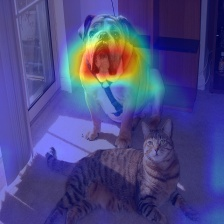
\includegraphics[width=4cm]{data/gradcam.jpg}
            };
        }
        \visible<8-14>{
            \node[] (imagefeatures) at (-3, 1) {
                \usebox{\largefeaturespaceconcept}
            };
        }
        \visible<8-15>{
            \node[] at (-2.75, -2.3) {
                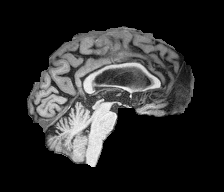
\includegraphics[width=2.5cm]{data/mri_sagittal.png}
            };
        }
        \visible<9-10>{
            \node[draw=black, text width=4cm, align=flush left] at (2.75, -2.3) {
                The patient shows cortical atrophy, reduced hippocampal volumes and enlarged ventricles
            };
        }
        \visible<10-12>{
            \node[] (textfeatures) at (2.5, 1) {
                \usebox{\largefeaturespacetext}
            };
        }
        \visible<11-15>{
            \node[draw=black, text width=4cm, align=flush left] (report) at (2.75, -2.3) {
                The patient shows \textcolor{red}{cortical atrophy}, reduced hippocampal volumes and enlarged ventricles
            };
            \draw[-stealth, red, thick] ($ (report) + (-0.8, 0.4) $) -- ($ (textfeatures.south) + (0.2, 0.1) $);
        }
        \visible<13-15>{
            \node[] (textfeatures) at (2.5, 1) {
                \usebox{\largefeaturespacetextred}
            };
        }
        \visible<14-15>{
            \draw[red, stealth-stealth, thick] ($ (imagefeatures.east) + (-0.47, 0.45) $) -- ($ (textfeatures.west) + (0.94, 0.45) $);
        }
        \visible<15>{
            \node[] (imagefeatures) at (-3, 1) {
                \usebox{\largefeaturespacelabel}
            };
        }
    \end{tikzpicture}
\end{frame}

\end{document}
